%%%%%%%%%%%%%%%%%%%%%%%%%%%%%%%%%%%%%%%%%
% Dreuw & Deselaer's Poster
% LaTeX Template
% Version 1.0 (11/04/13)
%
% Created by:
% Philippe Dreuw and Thomas Deselaers
% http://www-i6.informatik.rwth-aachen.de/~dreuw/latexbeamerposter.php
%
% This template has been downloaded from:
% http://www.LaTeXTemplates.com
%
% License:
% CC BY-NC-SA 3.0 (http://creativecommons.org/licenses/by-nc-sa/3.0/)
%
%%%%%%%%%%%%%%%%%%%%%%%%%%%%%%%%%%%%%%%%%

%----------------------------------------------------------------------------------------
%	PACKAGES AND OTHER DOCUMENT CONFIGURATIONS
%----------------------------------------------------------------------------------------

\documentclass[final,hyperref={pdfpagelabels=false}]{beamer}

\usepackage[orientation=portrait,size=a0,scale=1.4]{beamerposter} % Use the beamerposter package for laying out the poster with a portrait orientation and an a0 paper size

\usetheme{I6pd2} % Use the I6pd2 theme supplied with this template

\usepackage[english]{babel} % English language/hyphenation

\usepackage{amsmath,amsthm,amssymb,latexsym} % For including math equations, theorems, symbols, etc

%\usepackage{times}\usefonttheme{professionalfonts}  % Uncomment to use Times as the main font
%\usefonttheme[onlymath]{serif} % Uncomment to use a Serif font within math environments

\boldmath % Use bold for everything within the math environment

\usepackage{booktabs} % Top and bottom rules for tables

\graphicspath{{figures/}} % Location of the graphics files

\usecaptiontemplate{\small\structure{\insertcaptionname~\insertcaptionnumber: }\insertcaption} % A fix for figure numbering

%----------------------------------------------------------------------------------------
%	TITLE SECTION 
%----------------------------------------------------------------------------------------

\title{\huge Deep Learning
From Population Genomics \\
For Biological Evolution} % Poster title

\author{Karel Ha} % Author(s)

\institute{
Life Sciences -- Faculty of Natural Sciences\\
% Department of~Life Sciences\\
% Faculty of Natural Sciences\\
Imperial College London} % Institution(s)

%----------------------------------------------------------------------------------------
%	FOOTER TEXT
%----------------------------------------------------------------------------------------

\newcommand{\leftfoot}{business card: \href{http://q-r.to/bal4ks}{http://q-r.to/bal4ks}} % Left footer text

\newcommand{\rightfoot}{\href{mailto:k.ha19@ic.ac.uk}{k.ha19@ic.ac.uk}} % Right footer text

%----------------------------------------------------------------------------------------

\begin{document}

\addtobeamertemplate{block end}{}{\vspace*{2ex}} % White space under blocks

\begin{frame}[t] % The whole poster is enclosed in one beamer frame

\begin{columns}[t] % The whole poster consists of two major columns, each of which can be subdivided further with another \begin{columns} block - the [t] argument aligns each column's content to the top

\begin{column}{.02\textwidth}\end{column} % Empty spacer column

\begin{column}{.465\textwidth} % The first column

%----------------------------------------------------------------------------------------
%	OBJECTIVES
%----------------------------------------------------------------------------------------

\begin{block}{Objectives}

\begin{enumerate}
\item TODO
% \item Donec fringilla, velit id lobortis commodo, eros dui consectetur mi, ut interdum lorem dui sed mauris.
% \item Nulla ac nulla rhoncus est bibendum ullamcorper:
% \item Quisque vestibulum, nisl sit amet gravida ultricies dis parturient montes, nascetur ridiculus musobortis commodo, eros dui consectetur mi.
\end{enumerate}

\end{block}

%----------------------------------------------------------------------------------------
%	INTRODUCTION
%----------------------------------------------------------------------------------------
            
\begin{block}{Introduction}

\begin{itemize}
\item TODO
% \item Donec fringilla, velit id lobortis commodo, eros dui consectetur mi, ut interdum lorem dui sed mauris. Duis id sem nunc, a pharetra odio. Phasellus posuere \alert{semper massa}, id bibendum ligula tristique at. Integer sit amet vulputate turpis. Sed erat lacus, faucibus at viverra et, mattis nec sem. Cras faucibus \alert{scelerisque} cursus. Opet volutpat ligula. Duis semper lorem eget dui dignissim porttitor. Nulla facilisi. In ullamcorper lorem quis dolor iaculis nec egestas enim ultricies. Cras ut mauris elit, ut lacinia dui. Proin in ante et libero hendrerit iaculis. Nulla eu erat a urna laoreet auctor id a turpis. Nam mollis tristique neque eu luctus. Suspendisse rutrum congue nisi sed convallis. Aenean id neque dolor.
\end{itemize}

\end{block}

%----------------------------------------------------------------------------------------
%	METHODS
%----------------------------------------------------------------------------------------

\begin{block}{[TODO] Materials: Malaria Vector Mosquitoes}

\begin{columns} % Subdivide the first main column
\begin{column}{.4\textwidth} % The first subdivided column within the first main column
\begin{itemize}
\item TODO
\end{itemize}
\end{column}

\begin{column}{.6\textwidth} % The second subdivided column within the first main column
\centering

\begin{figure}
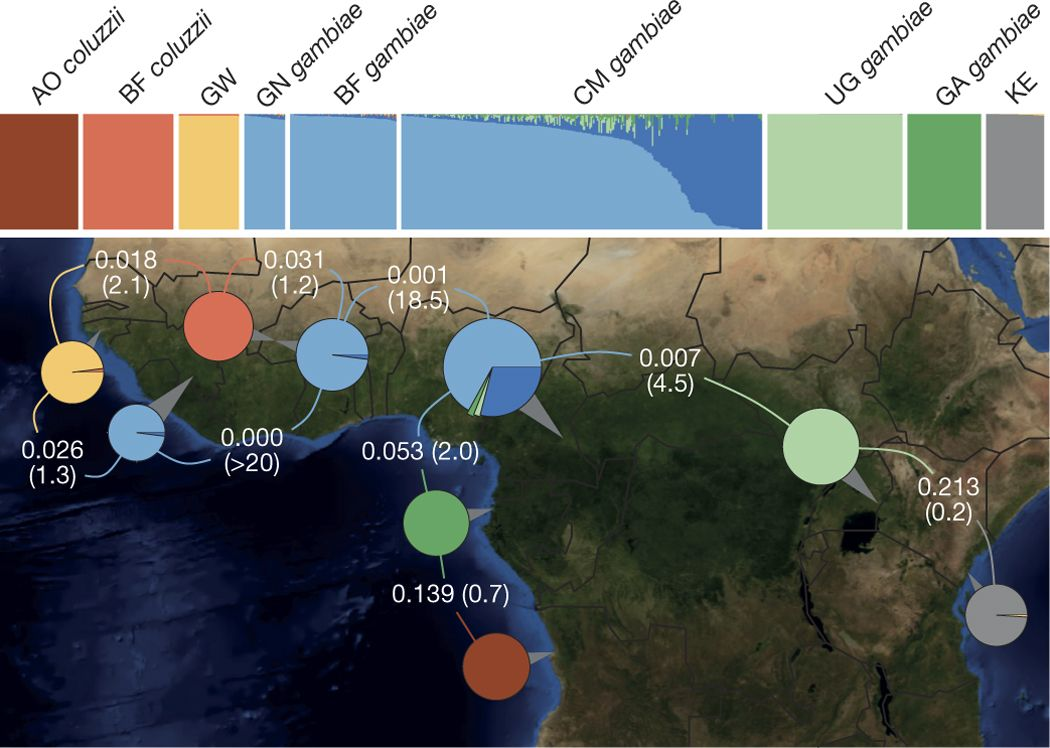
\includegraphics[width=.95\linewidth]{nature-mosquitoes/fig_2}
\caption{Geographical population structure and migration [TODO ref.]}
% Top, each mosquito is depicted as a vertical bar painted by the proportion of the genome inherited from each of K = 8 inferred ancestral populations. Pie charts on the map depict the same ancestry proportions summed over all individuals for each population. Text in white shows average fixation index (FST) followed in parentheses by estimates of the population migration rate (2Nm).
\end{figure}

\begin{figure}
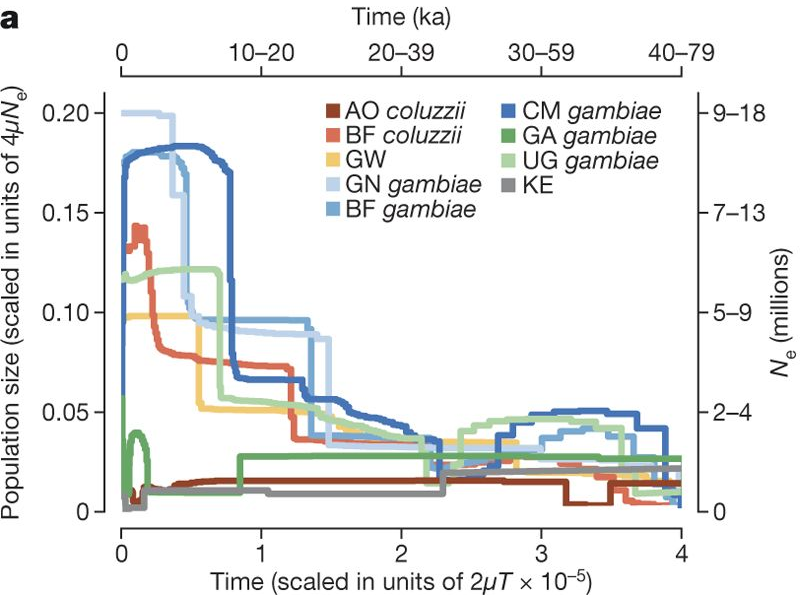
\includegraphics[width=.95\linewidth]{nature-mosquitoes/fig_3a}
\caption{Population size history [TODO ref.]}
% a, Stairway plot of changes in population size over time. Absolute values of time and Ne are shown on alternative axes as a range of values, assuming lower and upper limits for the mutation rate μ as 2.8 × 10−9 and 5.5 × 10−9, respectively, and t = 11 generations per year. ka, thousand years ago.
\end{figure}

\end{column}

\end{columns} % End of the subdivision
\end{block}

%------------------------------------------------

\begin{block}{[TODO] Insecticide Resistance}

\begin{figure}
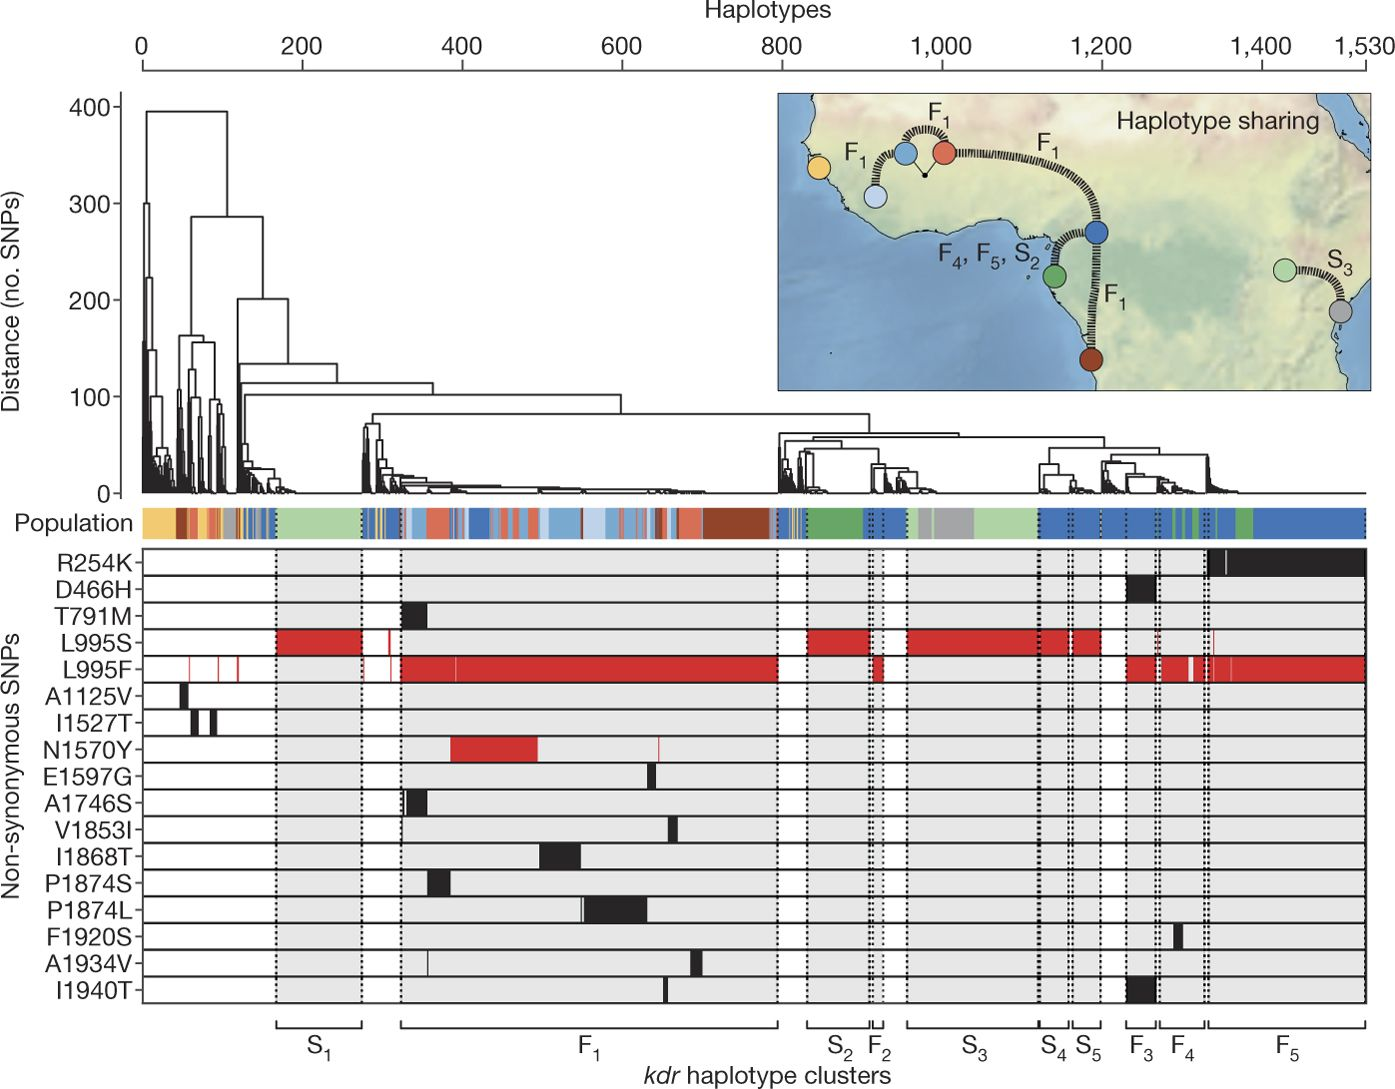
\includegraphics[width=.95\linewidth]{nature-mosquitoes/fig_4}
\caption{Evolution and spread of~insecticide resistance in~the \textit{Vgsc} gene [TODO ref.]}
% Top, a dendrogram obtained by hierarchical clustering of haplotypes from wild-caught individuals. The colour bar below shows the population of origin for each haplotype. Bottom, alleles carried by each haplotype at 17 non-synonymous SNPs with alternative allele frequency > 1% (white denotes reference allele; black denotes alternative allele; red denotes previously known resistance allele). At the lower margin, we label 10 haplotype clusters carrying a kdr allele (either Leu995Phe or Leu995Ser). The inset map depicts haplotypes that are shared between populations, demonstrating the spread of insecticide resistance.
\end{figure}

\end{block}

%----------------------------------------------------------------------------------------

\end{column} % End of the first column

\begin{column}{.03\textwidth}\end{column} % Empty spacer column
 
\begin{column}{.465\textwidth} % The second column

%----------------------------------------------------------------------------------------

%----------------------------------------------------------------------------------------
%	METHODS
%----------------------------------------------------------------------------------------

\begin{block}{[TODO] Methods: Deep Learning}

\begin{columns} % Subdivide the first main column
\begin{column}{.6\textwidth} % The first subdivided column within the first main column
\begin{itemize}
\item TODO
\end{itemize}
\end{column}

\begin{column}{.4\textwidth} % The second subdivided column within the first main column
\centering

\begin{figure}
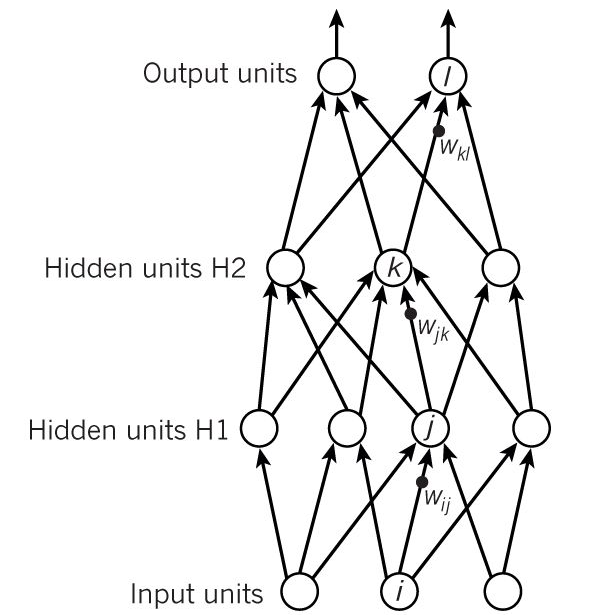
\includegraphics[width=.9\linewidth]{nature-deep-learning/fig_1c}
\caption{Multi-layer neural network [TODO ref.]}
% c, The equations used for computing the forward pass in a neural net with two hidden layers and one output layer, each constituting a module through which one can backpropagate gradients. At each layer, we first compute the total input z to each unit, which is a weighted sum of the outputs of the units in the layer below. Then a non-linear function f(.) is applied to z to get the output of the unit. For simplicity, we have omitted bias terms. The non-linear functions used in neural networks include the rectified linear unit (ReLU) f(z) = max(0,z), commonly used in recent years, as well as the more conventional sigmoids, such as the hyberbolic tangent, f(z) = (exp(z) − exp(−z))/(exp(z) + exp(−z)) and logistic function logistic, f(z) = 1/(1 + exp(−z)).
\end{figure}
\end{column}
\end{columns} % End of the subdivision

\begin{figure}
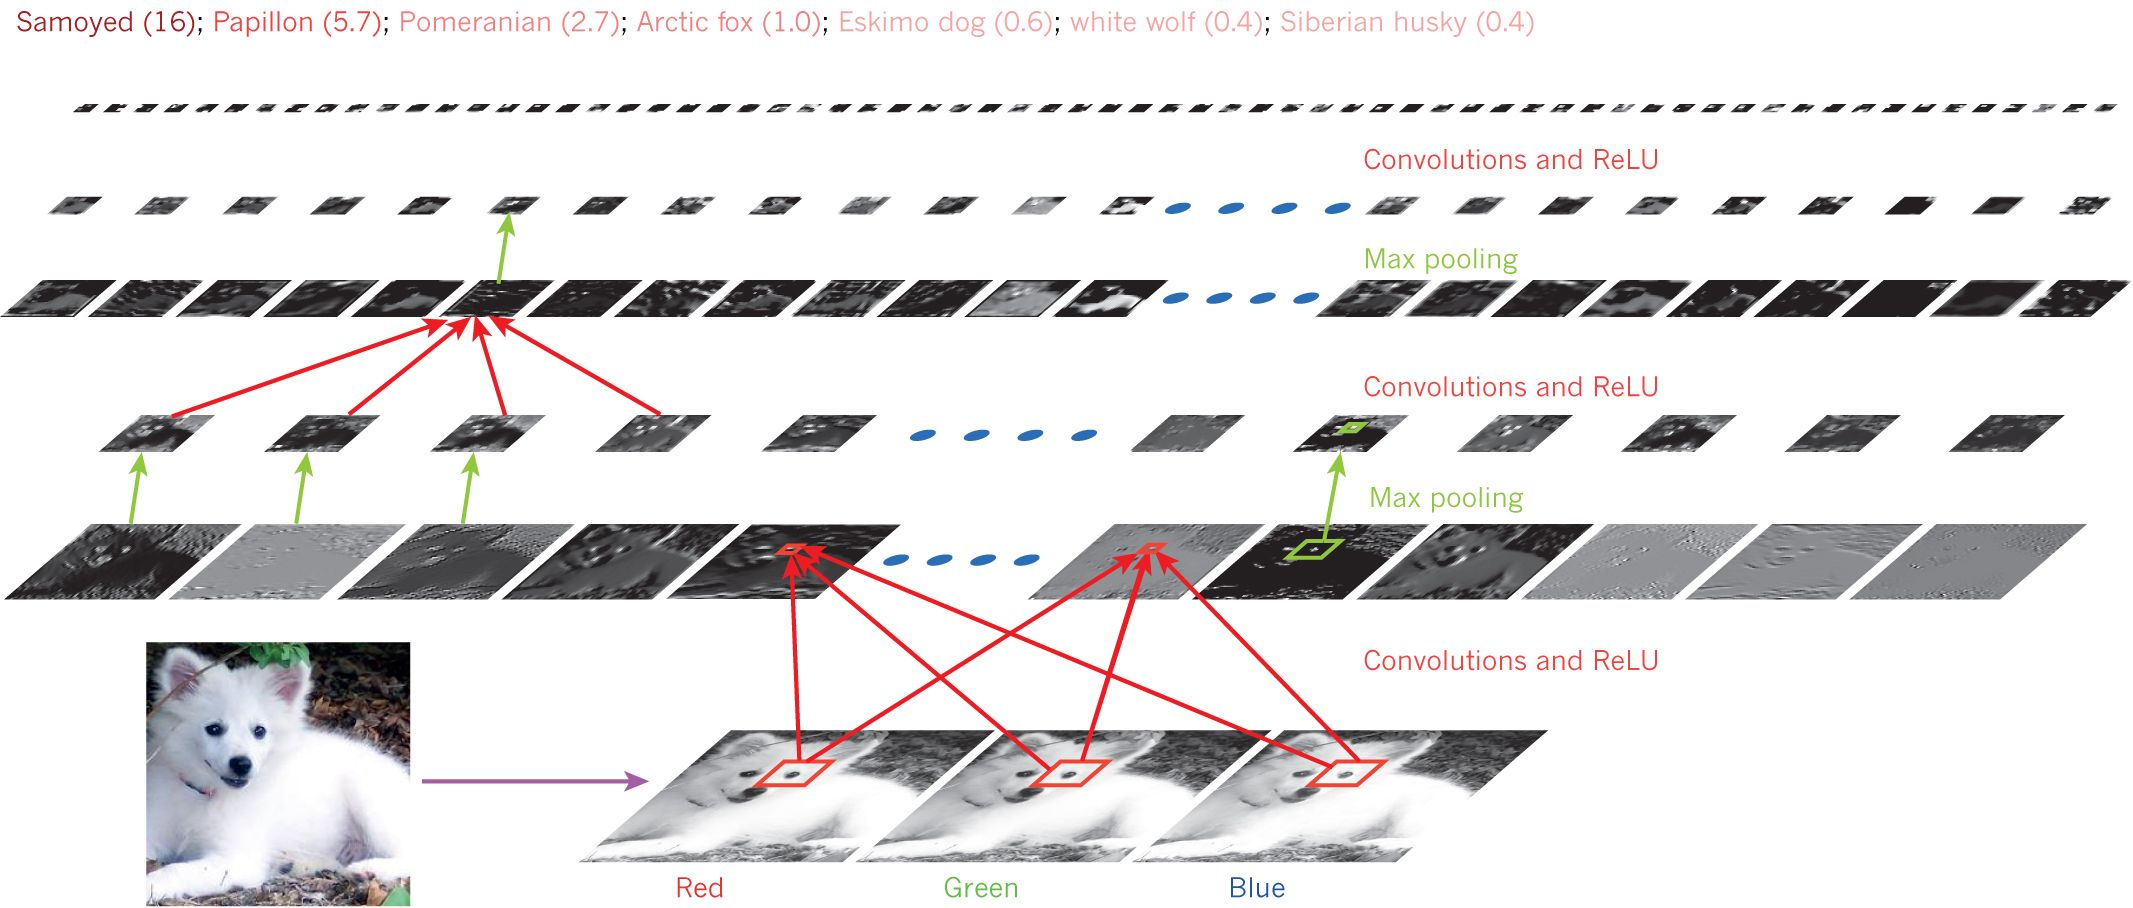
\includegraphics[width=.9\linewidth]{nature-deep-learning/fig_2}
\caption{Convolutional Neural Network [TODO ref.]}
% The outputs (not the filters) of each layer (horizontally) of a typical convolutional network architecture applied to the image of a Samoyed dog (bottom left; and RGB (red, green, blue) inputs, bottom right). Each rectangular image is a feature map corresponding to the output for one of the learned features, detected at each of the image positions. Information flows bottom up, with lower-level features acting as oriented edge detectors, and a score is computed for each image class in output. ReLU, rectified linear unit.
\end{figure}
\begin{itemize}
\item TODO
\end{itemize}

\begin{figure}
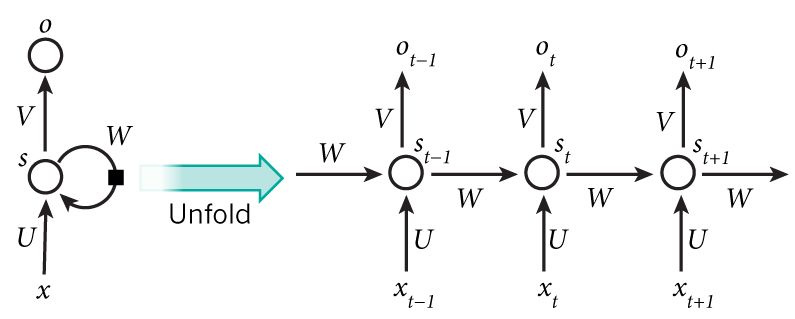
\includegraphics[width=.6\linewidth]{nature-deep-learning/fig_5}
\caption{Recurrent Neural Network [TODO ref.]}
% The artificial neurons (for example, hidden units grouped under node s with values st at time t) get inputs from other neurons at previous time steps (this is represented with the black square, representing a delay of one time step, on the left). In this way, a recurrent neural network can map an input sequence with elements xt into an output sequence with elements ot, with each ot depending on all the previous xt′ (for t′ ≤ t). The same parameters (matrices U,V,W) are used at each time step. Many other architectures are possible, including a variant in which the network can generate a sequence of outputs (for example, words), each of which is used as inputs for the next time step. The backpropagation algorithm (Fig. 1) can be directly applied to the computational graph of the unfolded network on the right, to compute the derivative of a total error (for example, the log-probability of generating the right sequence of outputs) with respect to all the states st and all the parameters.
\end{figure}
\begin{itemize}
\item TODO
\end{itemize}

\end{block}

%----------------------------------------------------------------------------------------
%	RESULTS
%----------------------------------------------------------------------------------------

% \begin{block}{Results: Table}

% \begin{itemize}
% \item TODO
% % \item Ased Aliquet Luctus Lectus
% \end{itemize}

% \begin{table}
% \begin{tabular}{l l l}
% \toprule
% \textbf{Treatments} & \textbf{Response 1} & \textbf{Response 2}\\
% \midrule
% Treatment 1 & 0.0003262 & 0.562 \\
% Treatment 2 & 0.0015681 & 0.910 \\
% Treatment 3 & 0.0009271 & 0.296 \\
% \bottomrule
% \end{tabular}
% \caption{Table caption}
% \end{table}

% \begin{itemize}
% \item Sollicitudin Vel Orci
% \item Maecenas Ultricies Feugiat Velit Non Mattis.
% \end{itemize}

% \begin{table}
% \begin{tabular}{l l l}
% \toprule
% \textbf{Treatments} & \textbf{Response 1} & \textbf{Response 2}\\
% \midrule
% Treatment 1 & 0.0003262 & 0.562 \\
% Treatment 2 & 0.0015681 & 0.910 \\
% Treatment 3 & 0.0009271 & 0.296 \\
% \bottomrule
% \end{tabular}
% \caption{Table caption}
% \end{table}
     
% \end{block}

%----------------------------------------------------------------------------------------
%	CONCLUSION
%----------------------------------------------------------------------------------------

\begin{block}{Conclusion}

\begin{itemize}
\item TODO
% \item Opet volutpat ligula. Duis semper lorem eget dui dignissim porttitor. Nulla facilisi. In ullamcorper lorem quis dolor iaculis nec egestas enim ultricies. Cras ut mauris elit, ut lacinia dui. Proin in ante et libero hendrerit iaculis.
% \item Nulla eu erat a urna laoreet auctor id a turpis. Nam mollis tristique neque eu luctus. Suspendisse rutrum congue nisi sed convallis. 
% \item Aenean id neque dolor.
% \item Opet volutpat ligula. Duis semper lorem eget dui dignissim porttitor. Nulla facilisi. In ullamcorper lorem quis dolor iaculis nec egestas enim ultricies. Cras ut mauris elit, ut lacinia dui. Proin in ante et libero hendrerit iaculis.
\end{itemize}

\end{block}

%----------------------------------------------------------------------------------------
%	REFERENCES
%----------------------------------------------------------------------------------------

\begin{block}{[TODO] References}
% TODO uncomment this?
% \nocite{*} % Insert publications even if they are not cited in the poster
\small{\bibliographystyle{unsrt}
\bibliography{sample}}

\end{block}

%----------------------------------------------------------------------------------------
%	ACKNOWLEDGEMENTS
%----------------------------------------------------------------------------------------

\begin{block}{Acknowledgments}

\begin{itemize}
\item TODO
% \item Nam mollis tristique neque eu luctus. Suspendisse rutrum congue nisi sed convallis. Aenean id neque dolor. Pellentesque habitant morbi tristique senectus et netus et malesuada fames ac turpis egestas.
\end{itemize}

\end{block}

%----------------------------------------------------------------------------------------
%	CONTACT INFORMATION
%----------------------------------------------------------------------------------------

\setbeamercolor{block title}{fg=black,bg=orange!70} % Change the block title color

\begin{block}{About Me}

\begin{columns} % Subdivide the first main column

\begin{column}{.65\textwidth} % The first subdivided column within the first main column
\begin{itemize}
\item \emph{computer science} background from Charles University (Prague, Czech Republic)
    \begin{itemize}
    \item algorithms
    \item applied mathematics
    \end{itemize}
    
\item co-supervised by:
    \begin{itemize}
	\item Dr Matteo Fumagalli (Quantitave Evolution lab)
	\item Prof. Austin Burt (Target Malaria consortium)
    \end{itemize}
    
\item previously
    \begin{itemize}
	\item in~academia: Charles University, EPFL$\dots$
	\item in~industry: IBM, CERN, H2O.ai$\dots$
    \end{itemize}
% \item Web: \href{http://www.university.edu/smithlab}{http://www.university.edu/smithlab}
% \item Email: \href{mailto:john@smith.com}{john@smith.com}
% \item Phone: +1 (000) 111 1111
\end{itemize}
\end{column}

\begin{column}{.35\textwidth} % The second subdivided column within the first main column
\centering
\begin{figure}

\includegraphics[width=0.95\linewidth]{figures/qr_Karel_Ha.png}
\end{figure}
\end{column}

\end{columns}

\end{block}

%----------------------------------------------------------------------------------------

\end{column} % End of the second column

\begin{column}{.015\textwidth}\end{column} % Empty spacer column

\end{columns} % End of all the columns in the poster

\end{frame} % End of the enclosing frame

\end{document}